\documentclass[12pt,a4paper,twoside]{article}
\usepackage[procnames]{listings}
\usepackage{fancyhdr}
\usepackage{lastpage}
\usepackage{a4wide} 
\usepackage{amsmath}
\usepackage{amssymb} 
\usepackage{graphicx}
\usepackage{color}
\usepackage{fancybox}
\usepackage{moreverb}
\usepackage{float}
\usepackage{dirtree}
\usepackage[T1]{fontenc}
% \usepackage{hangcaption}
\usepackage{listings}
\usepackage[utf8]{inputenc}
\title{IoT-LAB open node generic integration}
\author{ }
\date{July 2015}

\usepackage{natbib}
\usepackage{graphicx}

\begin{document}
\definecolor{keywords}{RGB}{255,0,90}
\definecolor{comments}{RGB}{0,0,113}
\definecolor{red}{RGB}{160,0,0}
\definecolor{green}{RGB}{0,150,0}
 
\lstset{language=Python, 
        basicstyle=\ttfamily\small, 
        keywordstyle=\color{keywords},
        commentstyle=\color{comments},
        stringstyle=\color{red},
        showstringspaces=false,
        identifierstyle=\color{green},
        procnamekeys={def,class}}

\maketitle

\section{Introduction}
The Iot-LAB experimental platform allow users to conduct remote experiments on wireless sensor board (such as an arduino board with an Xbee module).
For this purpose,a board called \textit{open-node}, can be connected to the IoT-LAB gateway, via the usb port.\newline
Bellow, the picture of an open-node connected to a gateway.\newline
\begin{figure}[H]
\centering
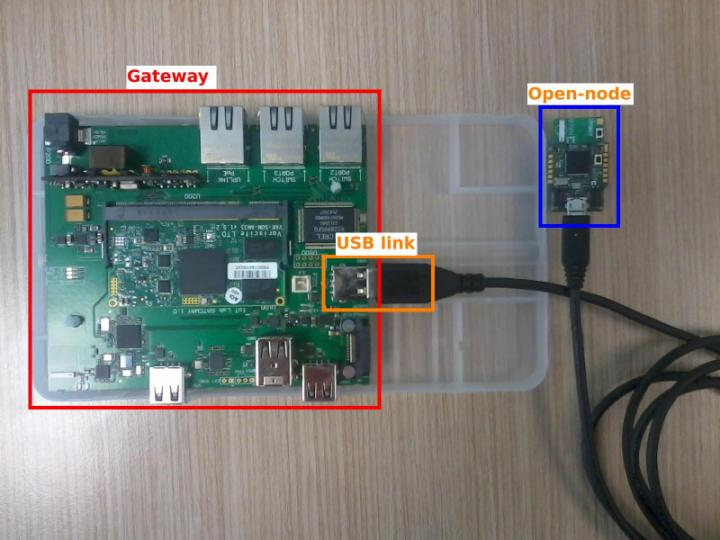
\includegraphics[scale=0.4]{gateway.jpg}
\caption{Gateway and wireless sensor board (e.g. Fox node)}
\label{fig1}
\end{figure}
On the linux distribution installed on the gateway, a Python module running provides a REST API able to receive remote commands to manage the open-node. The gateway can perform open-node commands like flashing a firmware in the open-node or starting his power supply on. \newline
This document show how to integrate a new open-node in the Iot-Lab platform.\newline
This integration is based on a plugin system provides by the Python module.
\section{Requirement}
Your node must be powered by USB.\newline
You must have developed at least two firmwares for your node : an autotest firmware and an idle firmware (describe in section bellow).\newline
\section{Adding a new open-node}
You can get the Python module code by cloning the git repository :
\begin{verbatim}
$git clone git@github.com:iot-lab/iot-lab-gateway.git
\end{verbatim}
\subsection{Module architecture}
This section present the module architecture.
\medskip
\dirtree{%
.1 bin/.
    .2 rules.d/.\DTcomment{ Directory for the udev rules}.
        .3 m3.rules.
        .3 a8.rules.
        .3 ....
.1 gateway-code/.
    .2 rest-server.py\DTcomment{ The API entry point}.
    .2 common.py.
    .2 gateway-manager.py.
    .2 autotest/\DTcomment{ Directory for all the autotest}.
    .2 utils/\DTcomment{ Contains script for serial operation such as serial redirection or programmer}.
        .3 avrdude.py.
        .3 openocd.py.
    .2 static/\DTcomment{ Contains the firmware and the configuration file}.
        .3 idle\_m3.elf.
        .3 m3\_autotest.elf.
        .3 iot-lab-m3.cnf.
        .3 ....
    .2 open\_nodes/\DTcomment{ Contains the code to interact with the open-node, you will put your code here}.
        .3 node\_a8.py.
        .3 node\_m3.py.
        .3 node\_fox.py.
        .3 node\_leonardo.py.
        .3 node\_mega.py.
}
\subsection{Udev rules}
Between two plugs, the name of the device as detected by the embedded linux running on the gateway can change : for example, an unique device can be succesively detected as ttyUSB0 and then as ttyUSB1.\newline 
As it is essential to have a fixed name for your device, you have to write a udev rules specific for your device.\newline
To do such a thing, you must create a file named your\_node.rules (with your\_node the name of your node).\newline
Using the command udevadm, you have to retrieve some information to identify your node such as the serial id, the id vendor or the id product. You must set a name for the device and set the right group (dialout) and the right mode (664). The convention is to name device ttyON\_NODENAME. \newline
Bellow the example of the udev rule for the node M3 : 

\begin{verbatim}
SUBSYSTEM=="tty", SUBSYSTEMS=="usb", ENV{ID_SERIAL}=="IoT-LAB_M3", 
ENV{ID_USB_INTERFACE_NUM}=="01",  SYMLINK+="ttyON_M3"

SUBSYSTEM=="usb", ATTR{idProduct}=="6011", ATTR{idVendor}=="0403", 
MODE="0664", GROUP="dialout"
\end{verbatim}
\subsection{Plugin integration}
\subsubsection{Naming convention}
As said previously, the application is based on a system of plugin : if you want to add a node, you just have to write a specific file to interface with the application.\newline
When the application is launched, the gateway take the name of your node located in the file \begin{verbatim}/var/local/config/board_type\end{verbatim} 
and then will use the class named Node\{nameofyournode\} located in \begin{verbatim}gateway-code/open_node/node_{nameofyournode}.py\end{verbatim}
to manage the expreriment. \newline
For example, if the name smt32nucleo is register on the gateway, the class used by the gateway will be 
\begin{verbatim}NodeStm32nucleo \end{verbatim}
in the file 
\begin{verbatim}gateway-code/open_node/node_stm32nucleo.py\end{verbatim}
If the name of your class or of your file not right formatted, an explicit error will be raised at the launch of the application.
\subsubsection{Interfacing the python code}
During the experiment and the tests, the application use several attributes located in your class. This attributes are the characteristic of your node and we can find for example, the name of your device as chosen in the udev rules (e.g. TTY); the baudrate which allow the communication between the gateway and your node (e.g. BAUDRATE).\newline
The list of the mandatory attributes are present in the template file in the annex. These attribute are required by the gateway for a good working.\newline
You can add your own attribute if needed by your class.\newline

The API provide services. These services are loaded dynamically, regarding what your open-node allow to do. These services are based on method implemented in your file : if the API need a specific method to create a service, the gateway-code will check if your class implement this method. If it doesn't, the service will not be available.

Some service are always available such as the start and stop of an experiment.
The method required by these service are mandatory and are the folowing :\newline
\begin{description}
\item[setup] \hfill \\ Perform all the action required to properly start an experiment.
\item[teardown] \hfill \\ Perform all the action required to properly stop an experiment.
\item[flash] \hfill \\ Flash a firmware on the open-node.
\end{description}
Others methods are not mandatory and can be implemented if you need them. The corresponding service will be available.
These functions are the following :
\begin{itemize}
\item debug\_start
\item debug\_stop
\item reset
\end{itemize}
A template file given in annex gather all the functions which interface with the code of the gateway.\newline
Here is a simple illustration of the execution of the start of the start\_exp command.\newline
\begin{figure}[H]
\centering
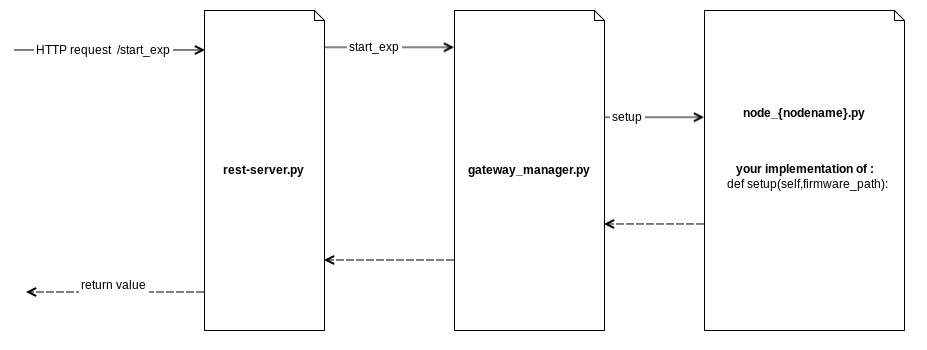
\includegraphics[scale=0.5]{diag.jpg}
\caption{Command execution diagram}
\label{fig1}
\end{figure}

Do not hesitate to watch the others implementation of open node to have a better idea of what the application expect.\newline

\subsubsection{Errors and return values}
When one of the function describe above terminate with a success, the return value must be 0.\newline
When the return value is different from 0, the application know that something gone wrong.\newline
Except status, all the method in the template file return an error.

\subsubsection{Flashing the open node}
Some method such as "reset", "flash" or "debug\_start", need to interact with the serial port of the open node. To do this, you will have to use a programmer software and write code to interact with it. Openocd and Avrdude are already available but maybe you will need to use another programmer and implement your own python file in the folder /gateway\_code/utils/.  
\subsection{Writing firmwares}
To add your code in the IoT-Lab platform, you must have writen two firmware.
These firmware must be put in the folder /gateway\_code/static/ as shown by the directory architecture.
\subsubsection{Idle firmware}
The idle firmware, must be a program with a consumption as low as possible (no led blinking, and no infinite loop). This firmware is flashed on the open node when no experiment are running.
\subsubsection{Autotest firmware}The autotest firmware is used during the testing phase. IotLAB-platform allow you to perform autotests for your device. It could be useful to see if the sensor on your node are still alive and send valid datas.\newline
During the testing phase, the gateway will flash the autotest firmware on the open-node and will then send some commands to the open-node. The gateway will expect the open-node to answer these command. For example, if your node embeds a light sensor, the gateway will send the following command on the serial port : \texttt{get\_light}. Your autotest firmware will receive this order, ask to the light sensor a measure and then send back to the gateway : \texttt{ACK get\_light value\_of\_measure lux}. Thanks to this, the gateway will know that the light sensor on your open-node is still working.\newline
A annex file gather all the autotest command which can be send by the gateway. In all these test, one is mandatory : the test\_echo. This test ensure that your open-node is still responding.\newline
The \texttt{echo} command must behave as describe bellow :
\begin{verbatim}
Gateway message : 'echo HELLO WORLD'
Node answer : 'HELLO WORLD'

Gateway message : 'echo ACK'
Node answer : 'ACK'
\end{verbatim}
To inform the application what kind of command your autotest firmware can handle, you must write the name of the test in the list AUTOTEST\_AVAILABLE as shown in the template file.\newline
When developing your implementation, it's possible to launch all the tests (and also the autotest) using the following command : \newline
\begin{verbatim}
fab -f tests_utils/integration_fabfile.py python_test -H adress-of-your-node
\end{verbatim}
\newpage
\section{Annex}
\subsection{template file}
Bellow you can find a template file which interface with the gateway application with proper comment, free to you to use it and modify it :
\begin{lstlisting}
# -*- coding:utf-8 -*-
""" Blank file for the implemention of an open-node called Nodename """

from gateway_code.config import static_path
from gateway_code import common
from gateway_code.common import logger_call

import logging
LOGGER = logging.getLogger('gateway_code')


class NodeNodename(object):

    TTY = '/dev/ttyON_NODENAME'
    # The tty as named in the udev rule
    BAUDRATE = 9600
    # The baudrate used to communicate with the open-node on the serial port
    FW_IDLE = static_path('idle_nodename.elf')
    # The name of the idle firmware
    FW_AUTOTEST = static_path('nodename_autotest.elf')
    # The name of the autotest firmware
    ALIM = '5V'
    # The tension of alimentation (will be 5V in most of the case)

    AUTOTEST_AVAILABLE = ['test_echo']
                        ]
    # The list of autotest available for your node.
    # As describe in the document, 
    # this list must contain at least 'test_echo'

    def __init__(self):
        # The initialization of your class

    @logger_call("Node Nodename : Setup of Nodename")
    def setup(self, firmware_path):
        # Here you will perform all the necessary action needed
        # by your node before the start of an experiment.
        return 1

    @logger_call("Node Nodename : teardown of nodename node")
    def teardown(self):
        # Here you will perform all the necessary action to
        # properly terminate your node
        return 1

    @logger_call("Node Nodename : flash of nodename node")
    def flash(self, firmware_path=None):
        # Here 
        return 1

    @logger_call("Node Nodename : reset of nodename node")
    def reset(self):
        # Not implemented
        return 1

    def debug_start(self):
        # Here you will start the debug of your node
        return 1

    def debug_stop(self):
        # Here you will stop the debug of your node
        return 1

    @staticmethod
    def status():
        # Here you will check your node (for exemple with ftdi chip)
        # if you are unable to check your node, just return 0
        return 0
        

\end{lstlisting}
\subsection{Autotests available}
Bellow you will find command that can be sent by the gateway during the tests and the corresponding format of the return expected.
\begin{description}
\item[test\_echo] \hfill \\ Format of the answer : already describe in the autotest section.
\item[test\_get\_time] \hfill \\ Format of the answer : ACK check\_get\_time 122953 tick\_32khz
\item[test\_uid] \hfill \\ Format of the answer : ACK get\_uid 05D8FF323632483343037109.
\item[test\_gyro] \hfill \\ Format of the answer : ACK get\_gyro 1.07625 1.75 5.2500002E-2 dps.
\item[test\_magneto] \hfill \\ Format of the answer : ACK get\_magneto 4.328358E-2 6.716418E-2 -3.880597E-1 gauss.
\item[test\_accelero] \hfill \\ Format of the answer : ACK get\_accelero 3.6E-2 -1.56E-1 1.0320001 g.
\item[test\_gpio] \hfill \\ Format of the answer : ACK test\_gpio.
\item[test\_i2c] \hfill \\ Format of the answer : ACK test\_i2c.
\item[test\_radio\_ping\_pong] \hfill \\ Format of the answer : ACK test\_radio\_ping\_pong.
\item[test\_radio\_with\_rssi] \hfill \\ Format of the answer : ACK test\_radio\_with\_rssi.
\item[test\_consumption\_dc] \hfill \\ Format of the answer : ACK test\_consumption\_dc.
\item[test\_leds\_with\_consumption] \hfill \\ Format of the answer : ACK test\_leds\_with\_consumption.
\item[test\_pressure] \hfill \\ Format of the answer : ACK get\_pressure 9.944219E2 mbar.
\item[test\_light] \hfill \\ Format of the answer : ACK get\_light 5.2001953E1 lux.
\item[test\_flash] \hfill \\ Format of the answer : ACK test\_flash.
\item[test\_gps] \hfill \\ Format of the answer : ACK test\_gps.
\item[test\_consumption\_batt] \hfill \\ Format of the answer : ACK test\_consumption\_batt.
\end{description}
\end{document}
